\documentclass[twocolumn]{article}
\usepackage[utf8]{inputenc}
\usepackage[T1]{fontenc}
\usepackage[polish]{babel}
\usepackage{amsmath, amssymb}
\usepackage{stfloats}
\usepackage{graphicx}
\usepackage{hyperref}
\usepackage{geometry}
\usepackage{algorithm}
\usepackage{algorithmic}
\usepackage{multicol}
\usepackage{float}
\floatname{algorithm}{Algorytm}
\geometry{margin=2.5cm}
\DeclareMathOperator*{\argmin}{arg\,min}
\newtheorem{definition}{Definicja}[section]
\title{Hierarchical Navigable Small World}
\author{Łukasz Jan Prus}
\date{24 Maj 2025}

\begin{document}

\maketitle

\begin{abstract}
Algorytm \textit{Hierarchical Navigable Small World} (HNSW) to jedna z najbardziej wydajnych metod typu przybliżonego wyszukiwania najbliższych sąsiadów (\textit{Approximate Nearest Neighbor} (ANN)). Jest ona wykorzystywana do szybkiego wyszukiwania podobieństw wektorowych (\textit{vector similarity search}) w przestrzeniach wysokowymiarowych. W niniejszej pracy przedstawiono szczegółową charakterystykę struktury HNSW, zasadę jej działania oraz sposób implementacji. Celem pracy jest kompleksowe zaprezentowanie HNSW jako narzędzia o wysokim potencjale w analizie danych.
\end{abstract}

\section{Wstęp teoretyczny}
Wektoryzacja danych jest jedną z najczęściej stosowanych metod przetwarzania różnorodnych danych zapisanych w systemach komputerowych. Wraz z rozwojem technologii oraz zwiększaniem pojemności pamięci masowych komputerów, bazy wektorowe rosną zarówno pod względem liczebności (liczba wektorów liczona w miliardach), jak i wymiarowości (liczba wymiarów przestrzeni liczona w setkach). 

W efekcie, tradycyjne algorytmy działające na tak liczebnych przestrzeniach wysokowymiarowych stają się niepraktyczne, ponieważ dokładne ich przeszukiwanie jest bardzo kosztowne obliczeniowo. Skutkuje to pojawieniem się nowego problemu algorytmicznego — wyszukiwania podobieństw wektorowych.

\subsection{Wyszukiwanie podobieństw wektorowych \newline \textit{(vector similarity search)}}
Przestrzeń wektorowa danych służy przede wszystkim do kategoryzacji danych. Podobne dane w poprawnie zbudowanej przestrzeni będą reprezentowane przez wektory, których poszczególne wymiary (cechy) różnią się nieznacznie. Oznacza to, że wektory o niewielkich odległościach\footnote{Metryka według której zdefiniowana jest funkcja odległości może być dowolna. Jej wybór jest zależny od sposobu wektoryzowania danych oraz pożądanych właściwości wyszukiwania.} reprezentują dane o podobnych cechach i odwrotnie.
\newline
Znalezienie podobnych danych sprowadza się do wybrania, bądź stworzenia wektora z pożądanymi cechami i znalezieniu najbliższych (najbardziej podobnych) do niego wektorów. Metoda ta jest szczególnie skuteczna w bardzo zagęszczonych bazach danych, to znaczy istnieje wiele wektorów w relatywnie niewielkich odległościach od poszukiwanego wektora.
\newline\newline
Formułując powyższy problem formalnie:

\begin{definition}\label{def:vector} \ \newline
Niech dana będzie przestrzeń wektorowa $\mathbb{R}^d$ oraz zbiór wektorów (baza danych) $\mathcal{D}$:
\[
\mathcal{D} = \{ \vec{x}_1, \vec{x}_2, \dots, \vec{x}_n \} \subset \mathbb{R}^d, \quad n,d \in \mathbb{N} 
\]
Dla zadanego zapytania $\vec{q} \in \mathbb{R}^d$ oraz określonej funkcji odległości $d : \mathbb{R}^d \times \mathbb{R}^d \to \mathbb{R}_{\geq 0}$, celem funkcji $f$ realizującej wyszukiwanie podobieństw wektorowych jest znalezienie $k$ wektorów z $\mathcal{D}$ najbardziej zbliżonych do $\vec{q}$, według tej funkcji odległości, gdzie:
\[
k \in \mathbb{N} \land k \leq \left|\mathcal{D}\right|
\]
\[
f_k: \mathbb{R}^d \to \left\{\mathcal{S} \subseteq \mathcal{D} : \left|\mathcal{S}\right| = k\right\}
\]
\[
f_k(\vec{q}) = \argmin_{\underset{\left|\mathcal{S}\right| = k}{\mathcal{S} \subseteq \mathcal{D}}} \ 
\sum_{\vec{x} \in \mathcal{S}} d\left(\vec{q}, \vec{x}\right)
\]
\end{definition} \ \newline
W przestrzeniach niskowymiarowych bardzo dobrze sobie radzą algorytmy oparte na binarnych drzewach przeszukiwań, między innymi k-d tree (k-dimensional tree), bądź ball tree. Algorytmy te jednak nie radzą sobie z przestrzeniami wysokowymiarowymi. Skutkuje to nowym podejściem do problemu. Zamiast próbować znaleźć dokładnego najbliższego sąsiada, co jest obliczeniowo niepraktyczne, algorytmy starają się oszacować jego położenie. Takie rozwiązanie nie zawsze znajdzie najbliższe wektory, ale znalezienie innego „bliskiego” wektora jest wystarczająco dobre w większości przypadków.

\subsection{Przybliżone wyszukiwanie najbliższych sąsiadów \newline \textit{(Approximate Nearest Neighbor)}}
Zamiast skupiać się na znalezieniu dokładnie najbliższych sąsiadów do wektora, ANN decyduje się na zmniejszenie dokładności w zamian za znaczne przyspieszenie przeszukiwania. Najczęściej budują one struktury danych, dzięki którym szacują, gdzie powinien znajdować się najbliższy wektor, a następnie obliczają funkcję odległości tylko dla części wszystkich wektorów. Ponieważ algorytmy te oparte są na elementach probabilistycznych, ich wyniki są niedeterministyczne, co może być postrzegane jako zaleta — dla tego samego zapytania mogą zostać zwrócone różne wyniki. W praktyce oznacza to, że zamiast tworzyć nowe zapytanie, wystarczy je ponowić, otrzymując w ten sposób wachlarz różnych wektorów wynikowych.
\newline
Algorytmy ANN działają heurystycznie, zatem nie spełniają definicji
\ref{def:vector}, gdyż nie zawsze ich zbiór wynikowy zawiera wszystkie $k$ najbliższych wektorów. Wprowadzono zatem nową miarę — tzw. recall. Recall to miara dokładności działania algorytmu dla danej przestrzeni, jest on opisany następującym wzorem
\[
\text{recall} = \frac{\left|\mathcal{S} \cap \mathcal{A}\right|}{k}
\]
Gdzie $\mathcal{S}$ to zbiór $k$ najbliższych sąsiadów spełniający definicję \ref{def:vector}, natomiast zbiór $\mathcal{A}$ to zbiór przybliżonych najbliższych sąsiadów zwrócony przez algorytm ANN. 
Istotne jest spostrzeżenie, że ze względu na niedeterministyczny charakter algorytmów ANN, wartość recall dla tego samego algorytmu i tej samej bazy danych może różnić się w kolejnych wywołaniach. Dlatego przy estymacji recall danego algorytmu zaleca się wykonanie wielu iteracji na zróżnicowanych próbkach przestrzeni wektorowej.
\vfill
\break
\section{Hierarchical Navigable Small World}
Hierarchical Navigable Small World (HNSW) to algorytm rozwiązujący problem wyszukiwania podobieństw wektorowych metodą przybliżonego wyszukiwania najbliższych sąsiadów (ANN). Wykorzystuje on wielopoziomową strukturę grafową opartą na właściwościach grafów małego świata (small-world graphs). Graf ten składa się z wielu warstw, gdzie każda kolejna wyższa warstwa zawiera coraz rzadsze połączenia między wierzchołkami, co pozwala na pokonanie problemu porzucania lokalnego optimum na rzecz znalezienia globalnego optimum.
\newline
Podczas wyszukiwania zapytanie rozpoczyna się na najwyższym poziomie, gdzie wykonywane jest heurystyczne przeszukiwanie wzdłuż krawędzi grafu. Następnie algorytm schodzi kolejno do niższych, gęstszych warstw, gdzie następuje dokładniejsze zawężenie obszaru poszukiwań. Takie podejście łączy efektywność przeszukiwania globalnego z precyzją lokalną, umożliwiając szybkie i dokładne znajdowanie przybliżonych najbliższych sąsiadów nawet na dużych i wysokowymiarowych zbiorach danych.
\newline\newline
Algorytm jest zbudowany na wielu parametrach, które istotnie wpływają na jego działanie. Owe parametry są wymienione i opisane pokrótce dla wygody czytelnika:
\begin{description}
  \item[$d$] liczba wymiarów wektorów w przestrzeni danych
  \item[$k$] liczba najbliższych sąsiadów zwracanych przez algorytm wyszukiwania
  \item[$m_L$] parametr normalizujący używany do próbkowania poziomu hierarchii
  \item[$M_{\max}$] maksymalna liczba krawędzi wychodzących z wierzchołka na poziomach wyższych niż 0
  \item[$M_{0\max}$] maksymalna liczba krawędzi wychodzących z wierzchołka na poziomie 0 (bazowym)
  \item[$\texttt{efConstruction}$] rozmiar listy kandydatów przeszukiwanych podczas dodawania nowego wierzchołka do grafu
\item[$\texttt{efSearch}$] rozmiar listy kandydatów przeszukiwanych podczas wyszukiwania $k$ najbliższych wierzchołków do wektora zapytania
\end{description}
\newpage
\subsection{Losowanie warstwy}
Pierwszym krokiem algorytmu Hierarchical Navigable Small World jest przypisanie każdemu punktowi poziomu (warstwy), do której będzie należał. Aby algorytm działał poprawnie liczba wektorów na wyższych warstwach musi być znacznie mniejsza niż liczba wektorów na warstwach niższych. W tym celu poziom $l$ dla danego punktu losowany jest zgodnie z wykładniczym rozkładem prawdopodobieństwa:
\begin{equation}\label{eq:l}
    l = \left\lfloor-\ln\left(\mathcal{U}\left(0,1\right)\right)\cdot m_L\right\rfloor \quad \cite{nmslib}
\end{equation}
Gdzie $m_{L}$ to parametr normalizujący, a $\mathcal{U}\left(0,1\right)$ to zmienna losowa o rozkładzie jednostajnym w przedziale $\left(0,1\right)$. Wartość parametru normalizującego ma wpływ na zachowanie struktury, zatem dobranie optymalnej wartości jest istotne. Typową wartością parametru jest $m_{L} = 1/\ln(M_{\max})$. \cite{Malkov2016}
\newline\newline
Przedstawienie zależności rozkładu punktów na warstwach od parametru $m_L$ obrazuje rysunek \ref{fig:1}. Niewielkie zmiany parametru drastycznie zmieniają rozkład. Można wykazać, że dla większego $m_L$ liczba poziomów w grafie będzie większa.

\begin{figure*}[!t]
    \centering
    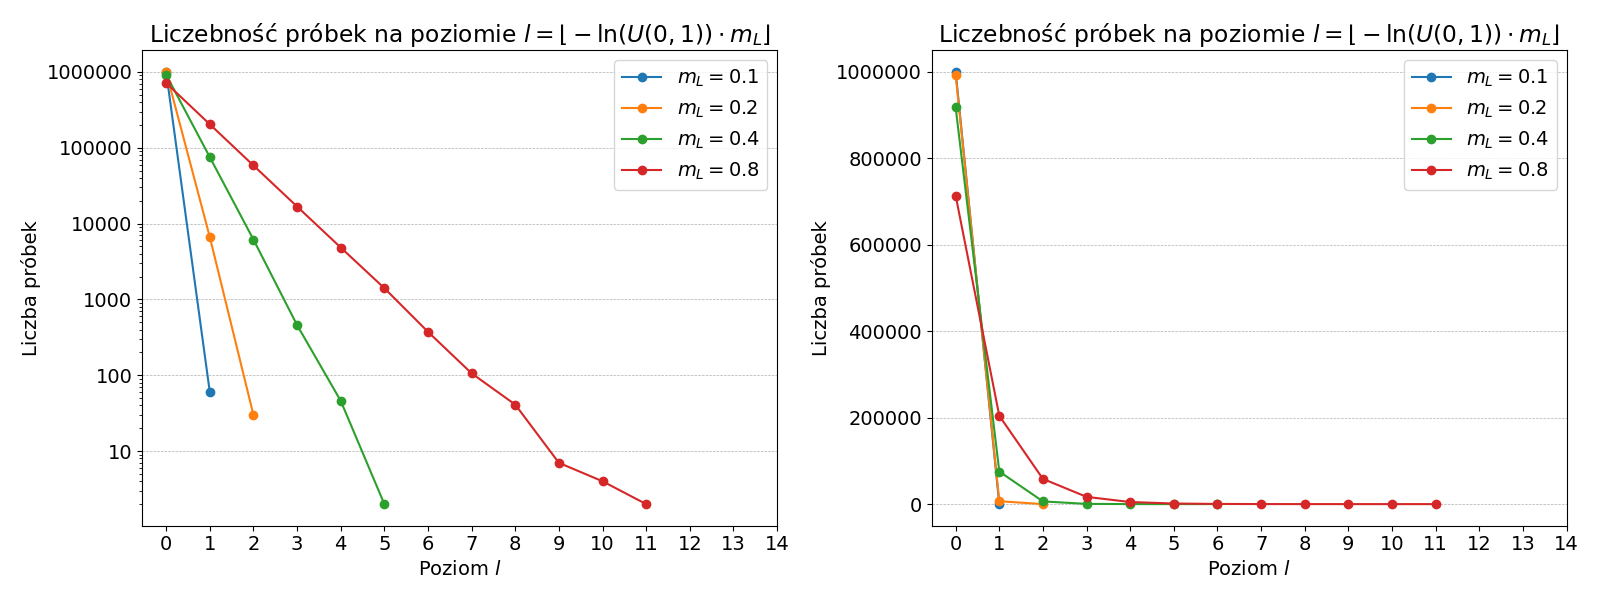
\includegraphics[width=1\linewidth]{Figure_1.png}
    \caption{Rozkład liczebności punktów na danym poziomie w zależności od parametru normalizującego $m_L$, w skalach linowej i logarytmicznej. Liczba punktów - 1 000 000.}
    \label{fig:1}
\end{figure*}
\vfill
\break
\subsection{Budowa grafów lokalnych dla poziomów}
Ten etap algorytmu to najbardziej obliczeniowo czasochłonny element całej implementacji, zatem wszelkie starania dążące do optymalizacji HNSW powinny skupiać się na tym elemencie.
Budowany graf to aproksymacja grafu Delaunay starający się minimalizować prawdopodobieństwo wystąpienia fałszywego globalnego minimum przy utrzymaniu jak najmniejszej liczby krawędzi między wierzchołkami \cite{Malkov2013}. Budowa tego grafu to sekwencyjna insercja elementów (Algorytm \ref{alg:insert}), gdzie dla każdego nowo stworzonego wierzchołka $q$ znajdujemy $\texttt{efConstruction}$ kandydatów na najbliższego sąsiada za pomocą wybranego algorytmu wyszukiwania, najczęściej greedy search (Algorytm \ref{alg:greedy}). Następnie z listy kandydatów wybieranych jest $M$ sąsiadów dla $q$, zazwyczaj jest to po prostu wybór $M$ najbliższych sąsiadów względem $q$ z podanego zbioru kandydatów, dlatego pomija się jego formalną definicję.
\newline
Warto zauważyć, że podczas przypisania wektorowi poziomu $l$, punkt ten występuje nie tylko w grafie warstwy $l$, ale także we wszystkich niższych warstwach $0\dots l-1$. Przedstawia to rysunek \ref{fig:2}.
\newpage

\begin{algorithm}[H]
\caption{Dodanie nowego wierzchołka \newline
INSERT($\texttt{HNSW}, q, M, M_{\max}, M_{0 \max},$ \newline $\makebox[4em][l]{\hfill} 
\texttt{efConstruction}, m_L)$ \newline
$q$ -- wektor, dla którego dodawany jest wierzchołek
}
\label{alg:insert}
\begin{algorithmic}[1]
\STATE $ep \leftarrow$ punkt na najwyższej warstwie grafu \texttt{HNSW}
\STATE $L \leftarrow$ numer najwyższej warstwy w grafie \texttt{HNSW}
\STATE $C \leftarrow \varnothing$ \COMMENT{lista kandydatów}
\STATE $l \leftarrow \left\lfloor -\ln\left(\mathcal{U}(0,1)\right) \cdot m_L \right\rfloor$ \COMMENT{równanie \eqref{eq:l}}

\FOR{$l_i = L, \dots, l+1$} 
    \STATE $C \leftarrow \text{SEARCH-LAYER}(q, ep, ef=1, l_i)$
    \STATE $ep \leftarrow$ element najbliższy do $q$ spośród $C$
\ENDFOR

\FOR{$l_i = \min(L, l), \dots, 0$}
    \STATE $C \leftarrow \text{SEARCH-LAYER}(q, ep,$ 
    \newline $\makebox[4em][l]{\hfill} \texttt{efConstruction}, l_i)$
    \STATE $N \leftarrow \text{SELECT-NEIGHBORS}(q, C, M, l_i)$
    \FOR{each $n$ in $N$}
        \STATE utwórz krawędź nieskierowaną między $q$ a $n$ w warstwie $l_i$
        \IF{$\deg(n) > M_{\max}$ \COMMENT{dla $l_i = 0$ użyj $M_{0\max}$}}
            \STATE $nN \leftarrow$ zbiór sąsiadów wierzchołka $n$ w warstwie $l_i$
            \STATE $nN \leftarrow \text{SELECT-NEIGHBORS}(n, nN, M, l_i)$
        \ENDIF
    \ENDFOR
    \STATE $ep \leftarrow$ $C$ \COMMENT{$ep$ zawiera teraz wszystkie punkty z $C$ jako punkty wejścia}
\ENDFOR

\IF{$l > L$}
    \STATE ustaw punkt startowy $ep$ w \texttt{HNSW} na $q$
\ENDIF
\end{algorithmic}
\end{algorithm}

\begin{algorithm}[H]
\caption{Wyszukanie kandydatów na sąsiadów metodą greedy search \newline
SEARCH-LAYER($\texttt{HNSW}, q, ep, ef, l_i$)
\newline $ef$ -- liczba kandydatów do zwrócenia
}
\label{alg:greedy}
\begin{algorithmic}[1]
\STATE $v \leftarrow \{ep\}$ \COMMENT{Zbiór odwiedzonych wierzchołków}
\STATE $C \leftarrow \{ep\}$ \COMMENT{Zbiór kandydatów do rozwinięcia}
\STATE $N \leftarrow \{ep\}$ \COMMENT{Zbiór najlepszych znalezionych sąsiadów}
\WHILE{$|C| > 0$}
    \STATE $c \leftarrow$ element najbliższy do $q$ spośród $C$
    \STATE $C \leftarrow C \setminus \{c\}$ \COMMENT{Usuń analizowany element z listy potencjalnych kandydatów}
    \STATE $f \leftarrow$ element najdalszy z $N$ względem $q$
    \IF{$\text{dist}(c, q) > \text{dist}(f, q)$}
        \STATE \textbf{break} \COMMENT{Nie znajdziemy już lepszych kandydatów}
    \ENDIF
    \FOR{każdy $n$ w sąsiedztwie($c$) w warstwie $l_i$}
        \IF{$n \notin v$}
            \STATE $v \leftarrow v \cup \{n\}$
            \STATE $f \leftarrow$ element najdalszy z $N$ względem $q$
            \IF{$|N| < ef$ \textbf{lub} $\text{dist}(n, q) < \text{dist}(f, q)$}
                \STATE $C \leftarrow C \cup \{n\}$
                \STATE $N \leftarrow N \cup \{n\}$
                \IF{$|N| > ef$}
                    \STATE $f \leftarrow$ element najdalszy z $N$ względem $q$
                    \STATE $N \leftarrow N \setminus \{f\}$ \COMMENT{Usuń najgorszy element}
                \ENDIF
            \ENDIF
        \ENDIF
    \ENDFOR
\ENDWHILE
\RETURN $N$
\end{algorithmic}
\end{algorithm}

\begin{figure}[H]
    \centering
    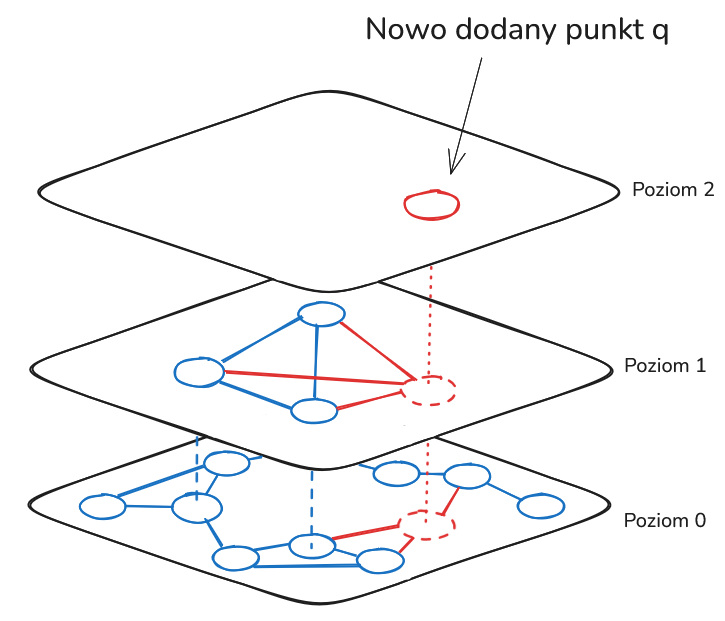
\includegraphics[width=1\linewidth]{Figure_2.png}
    \caption{Wizualizacja dodania punktu $q$ dla którego poziom $l$ jest równy 2, do grafu \texttt{HNSW}}
    \label{fig:2}
\end{figure}

\subsection{Wyszukiwanie najbliższych sąsiadów}
Interesującym aspektem algorytmu HNSW jest to, że wyszukiwanie zapytania przypomina procedurę dodawania nowego wierzchołka — wektor zapytania porusza się od najwyższej warstwy w dół, wykonując heurystyczne przeszukiwanie w każdej z warstw. Na najniższym poziomie (warstwie 0) zbierani są kandydaci, z których wybieranych jest $k$ najbliższych sąsiadów. W odróżnieniu od procedury dodawania, zapytanie nie modyfikuje struktury grafu. (Algorytm \ref{alg:knn})

\begin{algorithm}[H]
\caption{Wyszukanie kandydatów na sąsiadów metodą approximate kNN \newline
SEARCH-AkNN($\texttt{HNSW}, q, k, \texttt{efSearch}$)
}
\label{alg:knn}
\begin{algorithmic}[1]
\STATE $ep \leftarrow$ punkt na najwyższej warstwie grafu \texttt{HNSW}
\STATE $L \leftarrow$ numer najwyższej warstwy w grafie \texttt{HNSW}
\STATE $C \leftarrow \varnothing$ \COMMENT{lista kandydatów}
\FOR{$l_i \leftarrow L \dots 1$}
\STATE $C \leftarrow \text{SEARCH-LAYER}(\texttt{HNSW},$ \newline $ep, ef = 1, l_i)$
\STATE $ep \leftarrow$ element najbliższy do $q$ spośród $C$
\ENDFOR
\STATE $C \leftarrow \text{SEARCH-LAYER-GREEDY}(\texttt{HNSW},$ \newline $ep, ef = \texttt{efSearch}, l_i =0 )$
\RETURN $k$ elementów najbliższych do $q$ spośród $C$ 
\end{algorithmic}
\end{algorithm}

\begin{figure}[H]
    \centering
    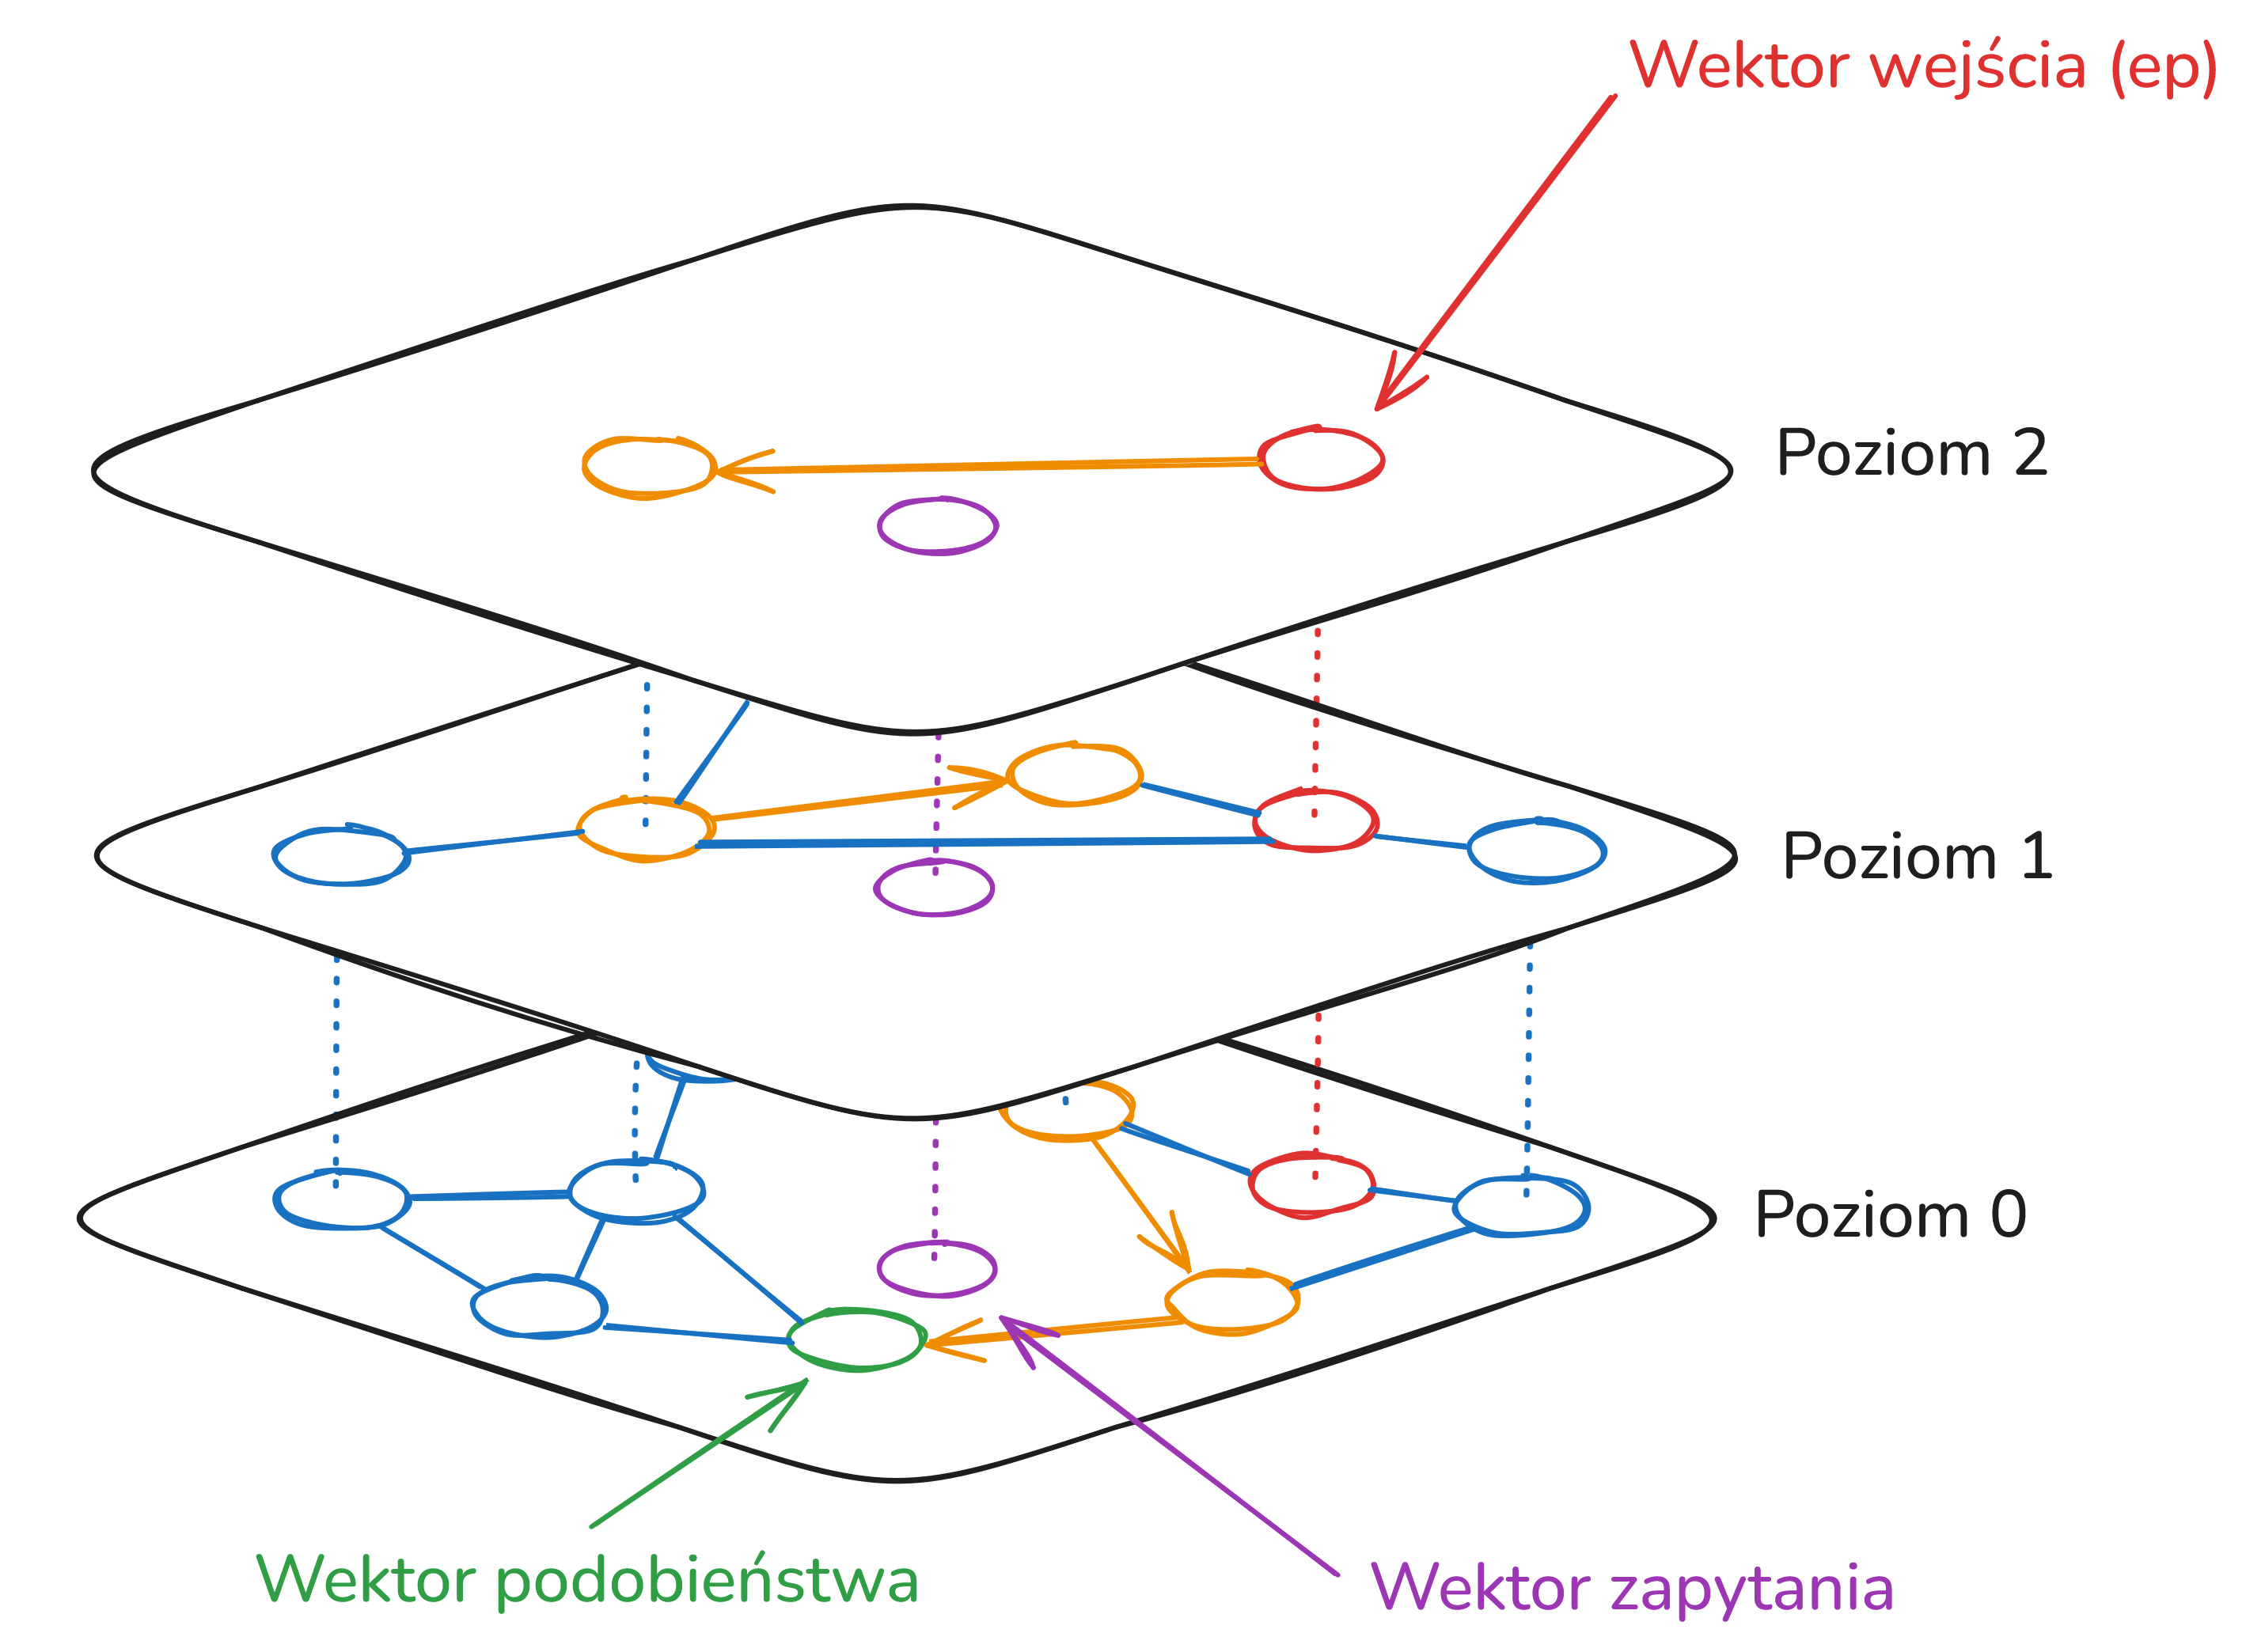
\includegraphics[width=1\linewidth]{Figure_3.png}
    \caption{Przebieg przeszukiwania zapytania w strukturze HNSW od poziomu 2 do 0 dla $k = 1$. Wektor wejścia ($ep$) reprezentuje punkt początkowy. Wynik (zielony) wskazuje na najbliższego sąsiada do wektora zapytania (fioletowy). Kolorem żółtym została oznaczona droga przeszukiwania oraz odwiedzone wierzchołki.}
    \label{fig:3}
\end{figure}

\subsection{Analiza złożoności}
\subsubsection{Analiza złożoności obliczeniowej wyszukiwania}
Złożoność obliczeniowa może być wyliczona przy założeniu, że graf budowany to graf Delaunay a nie jego przybliżenie, jednak jest ona wyznaczona empirycznie, co jest rozbieżne z zachowaniem HNSW przy wysokowymiarowych przestrzeniach. Według tej analizy złożoność obliczeniowa wynosi $O(log_2(N))$ \cite{Malkov2016}. W obecnym momencie analiza ta jest mało użyteczna, gdyż algorytm ten jest specyficznie używany dla wektorów wysokowymiarowych. Natura algorytmu, a w szczególności jego niedeterministyczność powodują, że dokładne matematyczne analizy złożoności są skomplikowane i niemarodajne (istnieją specjalne zbiory danych dla których złożoność wynosi $O(N)$) \cite{indyk2023worst}. Zatem ocenę szybkości algorytmu najlepiej przeprowadzać symulacyjnie, co w większości przypadków jest zgodne z oszacowaniem teoretycznym $O(log_2(N))$ bądź $O(N^\alpha)$ dla $\alpha \in [0.2, 0.4]$ \cite{Malkov2016}.
\newpage
\subsubsection{Analiza złożoności obliczeniowej budowania grafu}
Budowa grafu to iteratywne dodawanie wierzchołków, które sprowadza się do wykonania K-ANN search dla każdego poziomu \cite{Malkov2016}. Średnia liczba poziomów przypadających na pojedynczy wektor odpowiada wartości oczekiwanej ze wzoru \ref{eq:l}, powiększonej o 1. (Równanie \ref{eq:l} zwraca indeks a nie liczbę poziomów).
\begin{multline}
\text{$l$ to wartość skwantyfikowana} \\ \text{(przez użycie operatora zaokrąglenia w dół) zatem} \\
\mathbb{E}[l] = \sum_{i=0}^{\infty}i \cdot P(l = i) \\
\text{Z podstawowych przekształceń stochastycznych} \\
-\ln\left(\mathcal{U}\left(0,1\right)\right)\cdot m_L \sim Exp(1/m_{L}) \\
l = \left\lfloor Exp(1/m_{L}) \right\rfloor \\
\text{Zatem $P(l = i)$ przyjmuje postać} \\
P(i \leq Exp(1/m_{L}) < i+1) = \int_i^{i+1} \lambda e^{-\lambda x}dx \\
P(l = i) = \int_i^{i+1} m_L e^{-m_L x}dx = e^{-\frac{i}{m_L}} - e^{-\frac{i+1}{m_L}} \\
\text{Wartość oczekiwana przyjmuje postać} \\
\mathbb{E}[l] = \sum_{i=0}^{\infty}i \cdot (e^{-\frac{i}{m_L}} - e^{-\frac{i+1}{m_L}}) \\
\text{Średnia liczba poziomów} \\ \text{przypadająca na wektor wynosi} \\
\mathbb{E}[l] + 1  = 1 + \sum_{i=0}^{\infty}i \cdot (e^{-\frac{i}{m_L}} - e^{-\frac{i+1}{m_L}}) \\
\end{multline}
Powyższe równanie można porównać do złożoności obliczeniowej wyszukiwania \cite{Malkov2016}, zatem skaluje się ona jako $O(N \cdot \log_2(N))$.    

\subsubsection{Analiza złożoności pamięciowej}
Złożoność pamięciowa algorytmu HNSW to tak naprawdę rozmiar pamięci potrzebny na zapisanie zbudowanego grafu wielowarstwowego. Liczba połączeń dla elementów na poziomie bazowym to $M_{0 \max}$ natomiast dla pozostałych $M_{\max}$. Wiadomo, że $m_L$ to parametr normalizujący rozkład wykładniczy o parametrze 1, zatem $m_L$ określa średni poziom wierzchołka w grafie HNSW. Zatem średnie zużycie pamięci przez wierzchołek to:
\[
    (M_{0 \max} + M_{\max} \cdot m_{L}) \cdot \text{B}
\]
gdzie $B$ to liczba bajtów poświęcona na zapisanie połączenia. Uwzględniając, że współcześnie liczebność wektorowej bazy danych jest liczona w dziesiątkach miliardów (zakładając górne ograniczenie 50 miliardów). Wartości $M_{\max}$ są zazwyczaj w okolicach od 6 do 48 \cite{Malkov2016} zatem potrzeba dla zapisania pojedynczego połączenia (50 miliardów kombinacji), 5 bajtów razy liczbę połączeń (od 12 do 96) co daje szacunkowo od 60 do 480 bajtów. (Nie licząc pamięci potrzebnej na zapisanie danych wektorów). Powyższe oszacowanie jest zbieżne z przeprowadzonymi symulacjami \cite{Malkov2016}.

\section{Wnioski}

Algorytm HNSW stanowi jedną z najbardziej efektywnych metod wyszukiwania przybliżonych sąsiadów w dużych, wysokowymiarowych zbiorach danych. Dzięki wykorzystaniu grafów małego świata i hierarchicznej struktury, osiąga on kompromis między szybkością a dokładnością.

Potwierdzona efektywność HNSW czyni go wartościowym narzędziem w zastosowaniach takich jak analiza obrazu, systemy rekomendacyjne czy przetwarzanie języka naturalnego. Przyszłe prace mogą skupić się na automatyzacji doboru parametrów i integracji z systemami rozproszonymi.


\nocite{*}
\bibliographystyle{plain}
\bibliography{references}

\end{document}